\documentclass[11pt,a4paper]{article}
\usepackage{microtype}
\usepackage[margin=1in]{geometry}
\usepackage{setspace}
\usepackage{booktabs}
\usepackage{tabularx}
\usepackage{enumitem}
\usepackage[font=small,labelfont=bf,skip=6pt]{caption}
\usepackage{tikz}
\usetikzlibrary{positioning}
\usepackage[hidelinks]{hyperref}% load last
\captionsetup[table]{position=top}
\captionsetup[figure]{position=bottom}
\setstretch{1.15}
\setlength{\parindent}{0pt}
\setlength{\parskip}{0.6em}
\renewcommand{\arraystretch}{1.15}
\tikzset{
  >=stealth,
  block/.style={rectangle, rounded corners, draw, align=center,
    font=\footnotesize, minimum height=1.0cm},
}
\title{Vigil: Trust and Risk Intelligence for Mobile Money\\{\large AI Dev Fest 2026 AI Hackathon, Track 01}}
\author{Team JU\_MergeConflict\\Daffodil International University}
\date{October 2026}
\begin{document}
\maketitle

\section{Problem}

Mobile money runs on trust. In Bangladesh, wallets like upay move everyday
money for millions of people, and one scam call or one hijacked account can
wipe out a user's savings along with their faith in digital payments. Fraud
analysts fight this daily, but they drown in alerts. A typical system shows a
bare risk score with no explanation, so every serious case costs a long manual
investigation. Slow reviews mean stolen money keeps moving, analysts burn out,
and users leave the platform.

\section{Proposed idea}

Vigil is an AI investigation console that answers the three questions every
fraud case raises:
\begin{enumerate}[nosep]
  \item What happened?
  \item Why is it risky?
  \item What should upay do next?
\end{enumerate}
Each transfer is scored, the score is explained in plain auditable reasons and
mapped to a clear action, and the whole case is written up as a short
narrative in English or Bangla. High risk never blocks money on its own. It
holds the transaction, asks for step up authentication, and puts a human
analyst in charge.

\section{Implemented solution}

Figure~\ref{fig:arch} shows the full loop, which runs as three parts.

\begin{figure}[htbp]
\centering
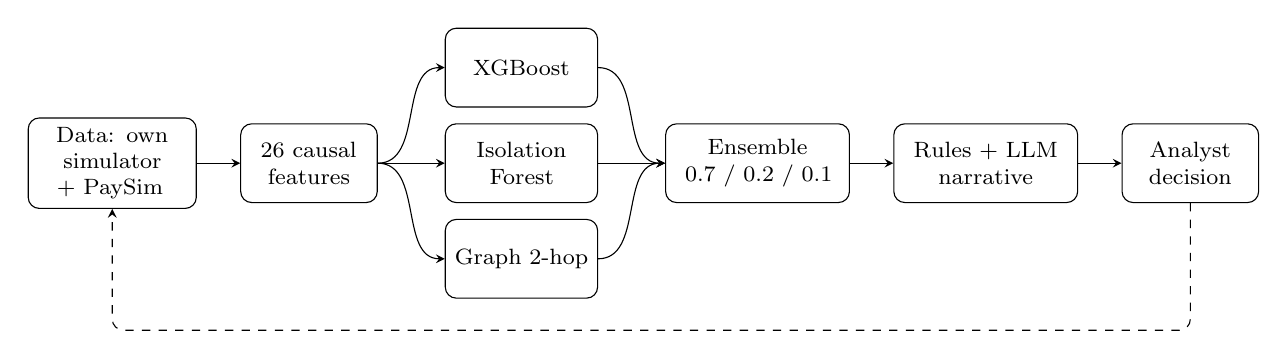
\begin{tikzpicture}[node distance=0.55cm]
  \node[block, text width=1.9cm] (data) {Data: own simulator + PaySim};
  \node[block, text width=1.5cm, right=of data] (feat) {26 causal features};
  \node[block, text width=1.7cm, right=0.85cm of feat] (iso) {Isolation Forest};
  \node[block, text width=1.7cm, above=0.2cm of iso] (xgb) {XGBoost};
  \node[block, text width=1.7cm, below=0.2cm of iso] (gr) {Graph 2-hop};
  \node[block, text width=2.1cm, right=0.85cm of iso] (ens) {Ensemble\\0.7 / 0.2 / 0.1};
  \node[block, text width=2.1cm, right=of ens] (narr) {Rules + LLM narrative};
  \node[block, text width=1.5cm, right=of narr] (act) {Analyst decision};
  \draw[->] (data) -- (feat);
  \draw[->] (feat.east) to[out=0,in=180] (xgb.west);
  \draw[->] (feat) -- (iso);
  \draw[->] (feat.east) to[out=0,in=180] (gr.west);
  \draw[->] (xgb.east) to[out=0,in=180] (ens.west);
  \draw[->] (iso) -- (ens);
  \draw[->] (gr.east) to[out=0,in=180] (ens.west);
  \draw[->] (ens) -- (narr);
  \draw[->] (narr) -- (act);
  \draw[->, dashed, rounded corners=4pt]
    (act.south) |- ([yshift=-0.4cm]gr.south) -| (data.south);
\end{tikzpicture}
\caption{Vigil pipeline, from data to analyst action with a retraining loop.}
\label{fig:arch}
\end{figure}

\begin{description}[nosep]
  \item[Scoring API (FastAPI).] A transfer arrives as sender, receiver,
    amount, device, location, and timestamp. The API returns a risk score
    between 0 and 1, a level of Low, Medium, or High, the top three reasons,
    a recommended action, and a written narrative, in about 25 milliseconds.
  \item[Analyst console (static web page).] A risk sorted queue with level
    filters and search, a case view with narrative, reasons, component
    scores, a mule ring panel, and a wallet timeline, plus a scoring
    playground and decision buttons that log Allow, Step up, or Freeze for
    future retraining.
  \item[Evaluation harness.] Measures the system on held out data and reports
    ranking quality, fairness across districts and account ages, latency, and
    business impact.
\end{description}
All development used synthetic data we generated ourselves plus public data,
following privacy by design. No production customer data was needed or used.

\section{Key features}

\begin{itemize}[nosep]
  \item Real time scoring with auditable top three reasons, backed by per
    transaction SHAP values.
  \item English and Bangla narratives with a deterministic offline fallback,
    so the demo works without internet.
  \item Mule ring discovery through the transaction graph, with fraud wallets
    near a receiver listed in each case.
  \item Strict input validation, isolated scoring traffic that cannot poison
    anyone's features, and a 47 test suite covering scoring, validation,
    security regressions, and the language model path.
  \item Thresholds in a config file, so new requirements integrate without
    retraining the models.
\end{itemize}

\section{AI approach}

\subsection{Data}

Table~\ref{tab:data} compares our two sources. Both are synthetic and contain
no real customer data. The difference that matters is authorship. Our
simulator injects scam, takeover, mule, and agent patterns of our own design,
plus realistic noise. PaySim is an independent public dataset collected from
Kaggle, built by other researchers with a simulator calibrated on aggregated
real logs. PaySim never trains the product. The retrained run below measures
pipeline portability; the frozen zero-shot runs in Table~\ref{tab:zeroshot}
test the trained weights themselves, with no refit.

\begin{table}[htbp]
\centering
\caption{Both datasets are synthetic. Only ours trains the product.}
\label{tab:data}
\begin{tabularx}{\textwidth}{@{}llrrX@{}}
\toprule
Source & Nature & Transactions & Fraud cases & Key signals \\
\midrule
Own simulator & Fully synthetic, ours & 50,000 & $\sim$2,000 & device, location, reset, velocity, graph \\
PaySim (Kaggle) & Synthetic, from real aggregates & 108,213 & 8,213 & amount, velocity, type, graph \\
\bottomrule
\end{tabularx}
\end{table}

\subsection{Models}

\begin{description}[nosep]
  \item[XGBoost classifier.] Learns fraud shapes from tens of thousands of
    labeled examples and outputs a probability of fraud.
  \item[IsolationForest.] Trained only on legitimate traffic, it flags behavior
    unlike anything normal, with scores calibrated to training percentiles.
  \item[Transaction graph.] Adds suspicion for receivers sitting near known
    fraud wallets, catching mule rings invisible to single transfers.
  \item[Ensemble.] A weighted blend of 0.7, 0.2, and 0.1 turns the three
    signals into one score, mapped to allow, review, or hold with human
    oversight.
\end{description}
A grounded language model narrates each case from the computed facts only,
under a fixed template with sanitized inputs.

\subsection{Evaluation}

Table~\ref{tab:eval} reports the same code with no tuning on both datasets.
On our data the system reaches 0.998 AUC against 0.81 for hand written rules.
On PaySim, where our best signals are unavailable, it holds 0.90 while the
rules collapse to a coin flip. We deliberately refused leakage features that
would have printed perfect scores and proved nothing.

Retraining shows the code works elsewhere; freezing the weights shows the
model itself travels. With no refit, the portable intersect model trained
only on cross-schema signals reaches 0.883 AUC and 0.786 recall at 5\%
FPR on PaySim, against 0.699 for full weights that lean on device signals
PaySim lacks --- evidence the portable design is what transfers. Two honest
limits: PaySim's chronological test window is 66\% fraud, so rank metrics
count and Precision@100 does not; and ranking transfers while operating
points do not, so bands are recalibrated per deployment
(docs/paysim-validation.md).

\begin{table}[htbp]
\centering
\caption{Same pipeline, same metrics, foreign data included.}
\label{tab:eval}
\begin{tabular}{@{}lrrrr@{}}
\toprule
Metric & Ours (model) & Ours (rules) & PaySim (model) & PaySim (rules) \\
\midrule
AUC & 0.9982 & 0.8119 & 0.8985 & 0.5049 \\
Precision@100 & 1.00 & 0.86 & 1.00 & 0.83 \\
Recall@5\%FPR & 0.9938 & 0.2149 & 0.6286 & 0.0000 \\
p95 latency & 25.9 ms & & 23.2 ms & \\
\bottomrule
\end{tabular}
\end{table}

\begin{table}[htbp]
\centering
\caption{Frozen weights, zero refit, PaySim test window.}
\label{tab:zeroshot}
\begin{tabular}{@{}lrr@{}}
\toprule
Metric & Intersect weights & Full weights \\
\midrule
AUC & 0.8829 & 0.6985 \\
Recall@5\%FPR & 0.7855 & 0.5957 \\
Frozen 0.60 band precision / recall & 0.67 / 0.95 & 0.67 / 0.95 \\
\bottomrule
\end{tabular}
\end{table}

\section{Intended real life impact}

\begin{itemize}[nosep]
  \item \textbf{Analysts:} a fifteen minute manual investigation becomes a two
    minute review, converted in our business simulation into loss prevented
    in BDT and analyst hours saved per thousand high risk holds.
  \item \textbf{Users:} faster holds on scams and takeovers stop stolen money
    sooner, and clear warnings protect first time and vulnerable customers
    before they pay a stranger.
  \item \textbf{upay:} every held scam is trust kept, and trust is what grows
    a wallet.
\end{itemize}
The API contract is stateless and ready to plug into a real stream, with
weekly retraining on governed labels as the path from prototype to pilot.
Responsible by design throughout: synthetic data only, explainable scores,
fairness measured, human oversight on every consequential action.

\end{document}
